% Options for packages loaded elsewhere
\PassOptionsToPackage{unicode}{hyperref}
\PassOptionsToPackage{hyphens}{url}
\PassOptionsToPackage{dvipsnames,svgnames,x11names}{xcolor}
%
\documentclass[
  10pt,
  ignorenonframetext,
]{beamer}
\usepackage{pgfpages}
\setbeamertemplate{caption}[numbered]
\setbeamertemplate{caption label separator}{: }
\setbeamercolor{caption name}{fg=normal text.fg}
\beamertemplatenavigationsymbolsempty
% Prevent slide breaks in the middle of a paragraph
\widowpenalties 1 10000
\raggedbottom
\setbeamertemplate{part page}{
  \centering
  \begin{beamercolorbox}[sep=16pt,center]{part title}
    \usebeamerfont{part title}\insertpart\par
  \end{beamercolorbox}
}
\setbeamertemplate{section page}{
  \centering
  \begin{beamercolorbox}[sep=12pt,center]{part title}
    \usebeamerfont{section title}\insertsection\par
  \end{beamercolorbox}
}
\setbeamertemplate{subsection page}{
  \centering
  \begin{beamercolorbox}[sep=8pt,center]{part title}
    \usebeamerfont{subsection title}\insertsubsection\par
  \end{beamercolorbox}
}
\AtBeginPart{
  \frame{\partpage}
}
\AtBeginSection{
  \ifbibliography
  \else
    \frame{\sectionpage}
  \fi
}
\AtBeginSubsection{
  \frame{\subsectionpage}
}
\usepackage{amsmath,amssymb}
\usepackage{iftex}
\ifPDFTeX
  \usepackage[T1]{fontenc}
  \usepackage[utf8]{inputenc}
  \usepackage{textcomp} % provide euro and other symbols
\else % if luatex or xetex
  \usepackage{unicode-math} % this also loads fontspec
  \defaultfontfeatures{Scale=MatchLowercase}
  \defaultfontfeatures[\rmfamily]{Ligatures=TeX,Scale=1}
\fi
\usepackage{lmodern}
\usetheme[]{Singapore}
\usefonttheme{serif}
\ifPDFTeX\else
  % xetex/luatex font selection
\fi
% Use upquote if available, for straight quotes in verbatim environments
\IfFileExists{upquote.sty}{\usepackage{upquote}}{}
\IfFileExists{microtype.sty}{% use microtype if available
  \usepackage[]{microtype}
  \UseMicrotypeSet[protrusion]{basicmath} % disable protrusion for tt fonts
}{}
\makeatletter
\@ifundefined{KOMAClassName}{% if non-KOMA class
  \IfFileExists{parskip.sty}{%
    \usepackage{parskip}
  }{% else
    \setlength{\parindent}{0pt}
    \setlength{\parskip}{6pt plus 2pt minus 1pt}}
}{% if KOMA class
  \KOMAoptions{parskip=half}}
\makeatother
\usepackage{xcolor}
\newif\ifbibliography
\setlength{\emergencystretch}{3em} % prevent overfull lines
\providecommand{\tightlist}{%
  \setlength{\itemsep}{0pt}\setlength{\parskip}{0pt}}
\setcounter{secnumdepth}{-\maxdimen} % remove section numbering
\newlength{\cslhangindent}
\setlength{\cslhangindent}{1.5em}
\newlength{\csllabelwidth}
\setlength{\csllabelwidth}{3em}
\newlength{\cslentryspacingunit} % times entry-spacing
\setlength{\cslentryspacingunit}{\parskip}
\newenvironment{CSLReferences}[2] % #1 hanging-ident, #2 entry spacing
 {% don't indent paragraphs
  \setlength{\parindent}{0pt}
  % turn on hanging indent if param 1 is 1
  \ifodd #1
  \let\oldpar\par
  \def\par{\hangindent=\cslhangindent\oldpar}
  \fi
  % set entry spacing
  \setlength{\parskip}{#2\cslentryspacingunit}
 }%
 {}
\usepackage{calc}
\newcommand{\CSLBlock}[1]{#1\hfill\break}
\newcommand{\CSLLeftMargin}[1]{\parbox[t]{\csllabelwidth}{#1}}
\newcommand{\CSLRightInline}[1]{\parbox[t]{\linewidth - \csllabelwidth}{#1}\break}
\newcommand{\CSLIndent}[1]{\hspace{\cslhangindent}#1}
\usepackage{multirow}
\ifLuaTeX
  \usepackage{selnolig}  % disable illegal ligatures
\fi
\IfFileExists{bookmark.sty}{\usepackage{bookmark}}{\usepackage{hyperref}}
\IfFileExists{xurl.sty}{\usepackage{xurl}}{} % add URL line breaks if available
\urlstyle{same}
\hypersetup{
  pdftitle={Module 10: Unsupervised learning (Overview/quizz lecture)},
  pdfauthor={Stefanie Muff, Department of Mathematical Sciences, NTNU},
  colorlinks=true,
  linkcolor={Maroon},
  filecolor={Maroon},
  citecolor={Blue},
  urlcolor={blue},
  pdfcreator={LaTeX via pandoc}}

\title{Module 10: Unsupervised learning (Overview/quizz lecture)}
\subtitle{TMA4268 Statistical Learning V2023}
\author{Stefanie Muff, Department of Mathematical Sciences, NTNU}
\date{March 23, 2023}

\begin{document}
\frame{\titlepage}

\begin{frame}[fragile]
\begin{block}{US Arrest Example}
\protect\hypertarget{us-arrest-example}{}
\(~\)

\begin{verbatim}
##            Murder Assault UrbanPop Rape
## Alabama      13.2     236       58 21.2
## Alaska       10.0     263       48 44.5
## Arizona       8.1     294       80 31.0
## Arkansas      8.8     190       50 19.5
## California    9.0     276       91 40.6
## Colorado      7.9     204       78 38.7
\end{verbatim}

\(~\)

Scales:

\begin{itemize}
\tightlist
\item
  Number of occurrence per 100 000 people
\item
  Percentage
\end{itemize}
\end{block}
\end{frame}

\begin{frame}[fragile]
\begin{block}{US Arrest Example}
\protect\hypertarget{us-arrest-example-1}{}
\(~\)

\begin{verbatim}
##            Murder Assault UrbanPop   Rape
## Alabama    0.0132   0.236       58 0.0212
## Alaska     0.0100   0.263       48 0.0445
## Arizona    0.0081   0.294       80 0.0310
## Arkansas   0.0088   0.190       50 0.0195
## California 0.0090   0.276       91 0.0406
## Colorado   0.0079   0.204       78 0.0387
\end{verbatim}

\(~\)

Scales:

\begin{itemize}
\tightlist
\item
  Number of occurrence per 100 people
\item
  Percentage
\end{itemize}

\(~\)

Scales:

\begin{itemize}
\tightlist
\item
  Number of occurrence per 100 people
\item
  Percentage
\end{itemize}
\end{block}
\end{frame}

\begin{frame}
\begin{block}{PC loadings vectors \(\Phi\)}
\protect\hypertarget{pc-loadings-vectors-phi}{}
\(~\)

\begin{table}

\centering
\begin{tabular}[t]{l|r|r|r|r}
\hline
  & PC1 & PC2 & PC3 & PC4\\
\hline
Murder & 0.0417 & -0.0448 & 0.0799 & -0.9949\\
\hline
Assault & 0.9952 & -0.0588 & -0.0676 & 0.0389\\
\hline
UrbanPop & 0.0463 & 0.9769 & -0.2005 & -0.0582\\
\hline
Rape & 0.0752 & 0.2007 & 0.9741 & 0.0723\\
\hline
\end{tabular}
\centering
\begin{tabular}[t]{l|r|r|r|r}
\hline
  & PC1 & PC2 & PC3 & PC4\\
\hline
Murder & 0.0000 & 0.0438 & -0.0680 & -0.9967\\
\hline
Assault & 0.0015 & 0.9968 & 0.0704 & 0.0390\\
\hline
UrbanPop & 1.0000 & -0.0015 & 0.0002 & -0.0001\\
\hline
Rape & 0.0003 & 0.0676 & -0.9952 & 0.0709\\
\hline
\end{tabular}
\end{table}

\(~\)
\end{block}
\end{frame}

\begin{frame}
\begin{block}{The biplot}
\protect\hypertarget{the-biplot}{}
\(~\)

\centering

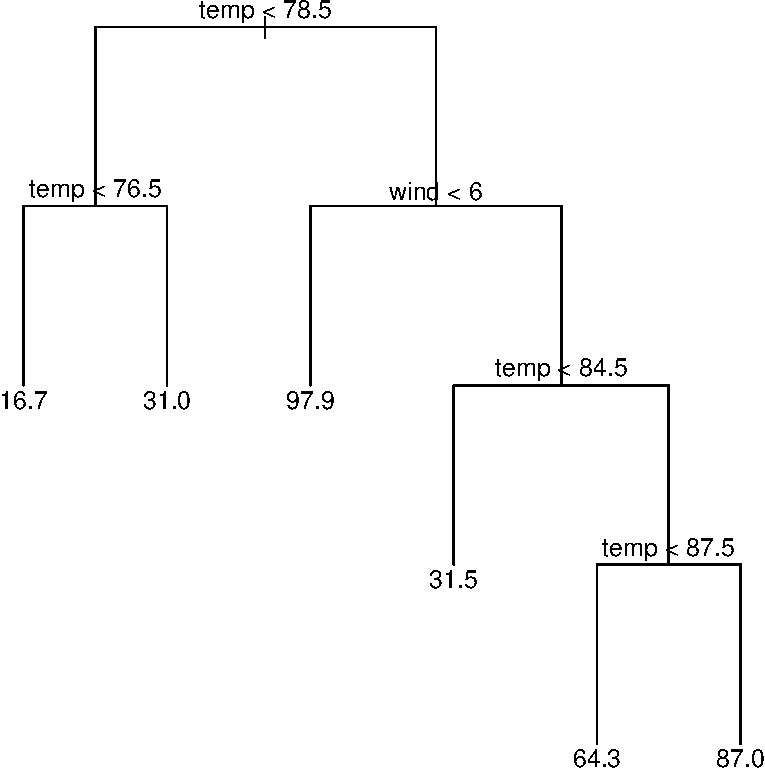
\includegraphics[width=0.4\linewidth]{10Unsuper_files/figure-beamer/unnamed-chunk-6-1}
\includegraphics[width=0.4\linewidth]{10Unsuper_files/figure-beamer/unnamed-chunk-6-2}
\end{block}
\end{frame}

\begin{frame}[fragile]
\begin{block}{Example from Compulsory 3, 2020}
\protect\hypertarget{example-from-compulsory-3-2020}{}
\(~\)

\begin{itemize}
\item
  We study the \texttt{decathlon2} dataset from the \texttt{factoextra}
  package in R, where Athletes' performance during a sporting meeting
  was recorded.
\item
  We look at 23 athletes and the results from the 10 disciplines in two
  competitions.
\end{itemize}

\(~\)

\scriptsize

\begin{verbatim}
##          100m long_jump shot_put high_jump  400m 110.hurdle discus pole_vault
## SEBRLE  11.04      7.58    14.83      2.07 49.81      14.69  43.75       5.02
## BERNARD 11.02      7.23    14.25      1.92 48.93      14.99  40.87       5.32
## YURKOV  11.34      7.09    15.19      2.10 50.42      15.31  46.26       4.72
##         javeline 1500m
## SEBRLE     63.19 291.7
## BERNARD    62.77 280.1
## YURKOV     63.44 276.4
\end{verbatim}
\end{block}
\end{frame}

\begin{frame}
\begin{figure}
\includegraphics[width=0.55\linewidth]{10Unsuper_files/figure-beamer/biplot-1} \end{figure}
\end{frame}

\begin{frame}
\begin{block}{Scree plot}
\protect\hypertarget{scree-plot}{}
\(~\)

A graphical description of the \textbf{proportion of variance explained
(PVE)} by a certain number of PCs (see Fig 12.3 from James et al.
(2013)):

\centering
\end{block}
\end{frame}

\begin{frame}
\begin{block}{Proportion of varianced explained (PVE)}
\protect\hypertarget{proportion-of-varianced-explained-pve}{}
\(~\)

\textbf{Recap:} The PVE by PC \(m\) is given by

\[
\frac{\sum_{i=1}^m z_{im}^2} {\sum_{j=1}^p\sum_{i=1}^n x_{ij}^2}
\]
\end{block}
\end{frame}

\begin{frame}{Clustering}
\protect\hypertarget{clustering}{}
\(~\)

\begin{itemize}
\item
  The aim is to find \emph{clusters} or \emph{subgroups}.
\item
  Clustering looks for homogeneous subgroups in the data.
\end{itemize}

\(~\)

Difference to PCA?

\pause

\(\rightarrow\) PCA looks for low-dimensional representation of the
data.
\end{frame}

\begin{frame}
\begin{block}{K-means vs.~hierarchical clustering}
\protect\hypertarget{k-means-vs.-hierarchical-clustering}{}
\(~\)

See menti.com
\end{block}
\end{frame}

\begin{frame}
\begin{block}{K-means clustering}
\protect\hypertarget{k-means-clustering}{}
\(~\)

\begin{itemize}
\tightlist
\item
  Fix the number of clusters \(K\).
\end{itemize}

\(~\)

\begin{itemize}
\tightlist
\item
  Find groups such that the sum of the within-cluster variation is
  minimized.
\end{itemize}

\(~\)

\begin{itemize}
\tightlist
\item
  Algorithm?
\end{itemize}
\end{block}
\end{frame}

\begin{frame}
\end{frame}

\begin{frame}
\centering

\flushleft
\small

(Fig 12.8 from course book)
\end{frame}

\begin{frame}
\begin{block}{Hierarchical clustering}
\protect\hypertarget{hierarchical-clustering}{}
\(~\)

Bottom-up agglomerative clustering that results in a
\emph{\textcolor{red}{dendogram}}.

\(~\)
\end{block}
\end{frame}

\begin{frame}
\begin{block}{Important in hierarchical clustering}
\protect\hypertarget{important-in-hierarchical-clustering}{}
\(~\)

\begin{itemize}
\tightlist
\item
  \emph{\textcolor{red}{Linkage:}} Complete, single, average centroid.
\end{itemize}

\(~\)

\begin{itemize}
\tightlist
\item
  \emph{\textcolor{red}{Dissimilarity measure:}} Euclidian distance,
  correlation. \emph{Other similarity/distance measures?}
  \footnote{ Note: Correlation is actually a similarity measure, not a distance measure. Implication?}
\end{itemize}
\end{block}
\end{frame}

\begin{frame}
\begin{block}{Hierarchical clustering -- example}
\protect\hypertarget{hierarchical-clustering-example}{}
\(~\)

Note: The representation on the right is not possible in
high-dimensional space (i.e., if we have \(X_1, X_2, X_3, ...., X_p\)).
\end{block}
\end{frame}

\begin{frame}
\begin{block}{Hierarchical clustering -- example}
\protect\hypertarget{hierarchical-clustering-example-1}{}
\(~\)

An exam question from 2022:
\end{block}
\end{frame}

\begin{frame}
\begin{block}{Pros and cons of clusterization methods / practical
issues}
\protect\hypertarget{pros-and-cons-of-clusterization-methods-practical-issues}{}
\(~\)

\(~\)

\(~\)

\(~\)

\(~\)

\(~\)

\(~\)

\(~\)

\(~\)

\(~\)
\end{block}
\end{frame}

\begin{frame}{References}
\protect\hypertarget{references}{}
\hypertarget{refs}{}
\begin{CSLReferences}{1}{0}
\leavevmode\vadjust pre{\hypertarget{ref-ISL}{}}%
James, Gareth, Daniela Witten, Trevor Hastie, and Robert Tibshirani.
2013. \emph{An Introduction to Statistical Learning}. Vol. 112.
Springer.

\end{CSLReferences}
\end{frame}

\end{document}
